\documentclass[12pt,letterpaper]{article}
\usepackage[utf8]{inputenc}
\usepackage{amsmath}
\usepackage{amsfonts}
\usepackage{amssymb}
\usepackage{amsthm}
\usepackage{graphicx}
\usepackage{tabularx}
\usepackage[left=2cm,right=2cm,top=2cm,bottom=2cm]{geometry}
\usepackage{fancyhdr}
\usepackage{multicol}
\usepackage{multirow,array}
\usepackage{newtxtext,newtxmath}
\usepackage{relsize}
\usepackage{lastpage}
\usepackage{cancel}
\usepackage{tikz}
\usepackage{enumitem}
\usepackage{adjustbox}
\newcolumntype{Y}{>{\centering\arraybackslash}X}
	\setenumerate[1]{label={\bf Q\theenumi: ~}}
	\setenumerate[2]{label={\bf \theenumii: ~}}
\pagestyle{fancy}
\fancyhf{}
\lhead{\textsc{BHCC Mat-181}}
\rhead{\textsc{Bayes' Theorem}}
\rfoot{Page \thepage ~of \pageref{LastPage}}

\newcommand*\circled[1]{\tikz[baseline=(char.base)]{
            \node[shape=circle,draw,inner sep=2pt] (char) {#1};}}

\begin{document}
\begin{enumerate}
\item Given:
\begin{align*}
P(A) &= 0.7 \\
P(B|A) &= 0.4 \\
P(B|A^c) &= 0.5
\end{align*}
\begin{enumerate}
\item Create a tree diagram to find all the joint probabilities.
\vfill
\item Make a contingency table.
\vfill
\newpage
\item Using the grid, draw a quantitative Venn diagram.
\begin{center}
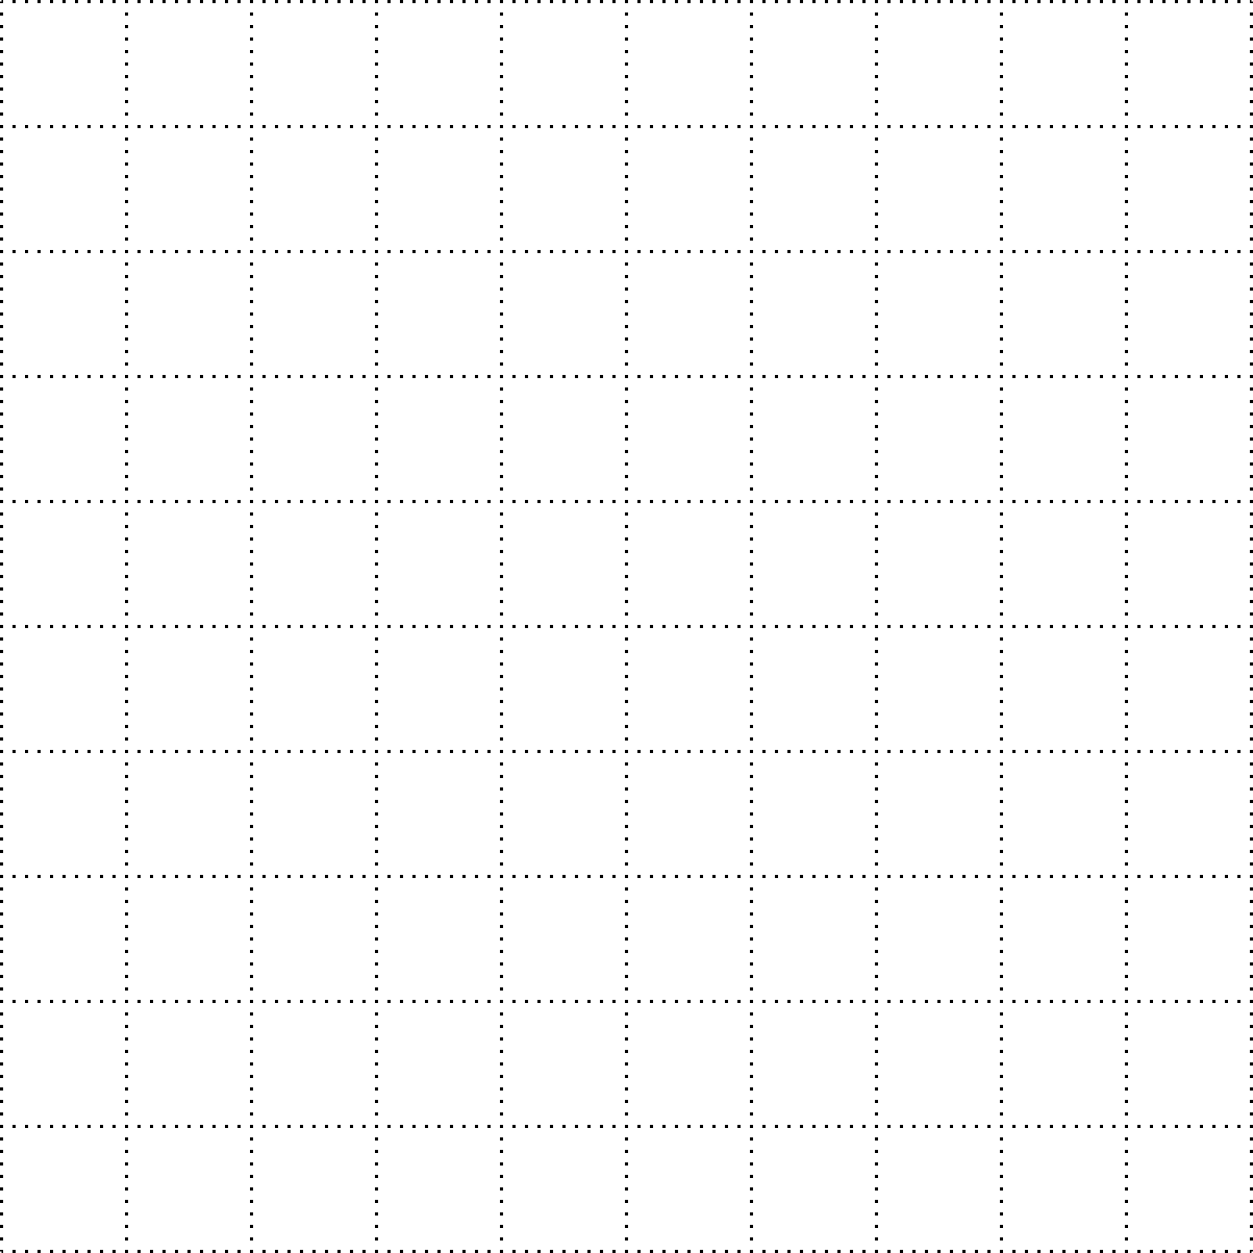
\includegraphics[scale=0.9]{figures/grid.png}
\end{center}
\item $P(B)= ?$
\vfill
\item $P(A ~\textsc{and}~B) = ?$
\vfill
\item $P(A^c ~\textsc{and}~B) = ?$
\vfill
\item $P(A ~\textsc{or}~B) = ?$
\vfill
\item $P(A|B) = ?$
\vfill
\item $P(A|B^c) = ?$
\vfill

\end{enumerate}
\end{enumerate}
\end{document}

